%!TEX root = ../thesis.tex
%*******************************************************************************
%****************************** Third Chapter **********************************
%*******************************************************************************
\chapter{Results}

% **************************** Define Graphics Path **************************
\ifpdf
    \graphicspath{{Chapter3/Figs/Raster/}{Chapter3/Figs/PDF/}{Chapter3/Figs/}}
\else
    \graphicspath{{Chapter3/Figs/Vector/}{Chapter3/Figs/}}
\fi

% Talk about ... in this section
This section presents the results of the simulation and gives some analysis and discussion about the results. An analysis of the trace statistics is given first, including trace lengths and trace composition (conditional branches and single-direction branches). Immediately afterwards the simulation results are compared between the trace sets and some useful WSC trace features are obtained, inspiring some thoughts on the causes of the prediction accuracy under the WSC workload. In the third section TAGE\cite{seznec_tage-sc-l_2016, seznec_exploring_2016} (SOTA) and some other predictors \cite{pruett_dynamically_2016, jimenez_multiperspective_2016-1, jimenez_multiperspective_2016} are compared. Finally, a review of the completion of the project is given and limits are discussed in detail.

% Section 3.1 Trace stat
\section{Traces statistics}

When studying new trace sets, it is natural and necessary to first study the statistical properties of the sets themselves. The four WSC sets (\textit{delta, whiskey, charlie} and \textit{merced}) show significant differences from each other, indicating that WSC workload branch traces strongly depend the application run on WSC.


\begin{figure}[h!] 
\centering    
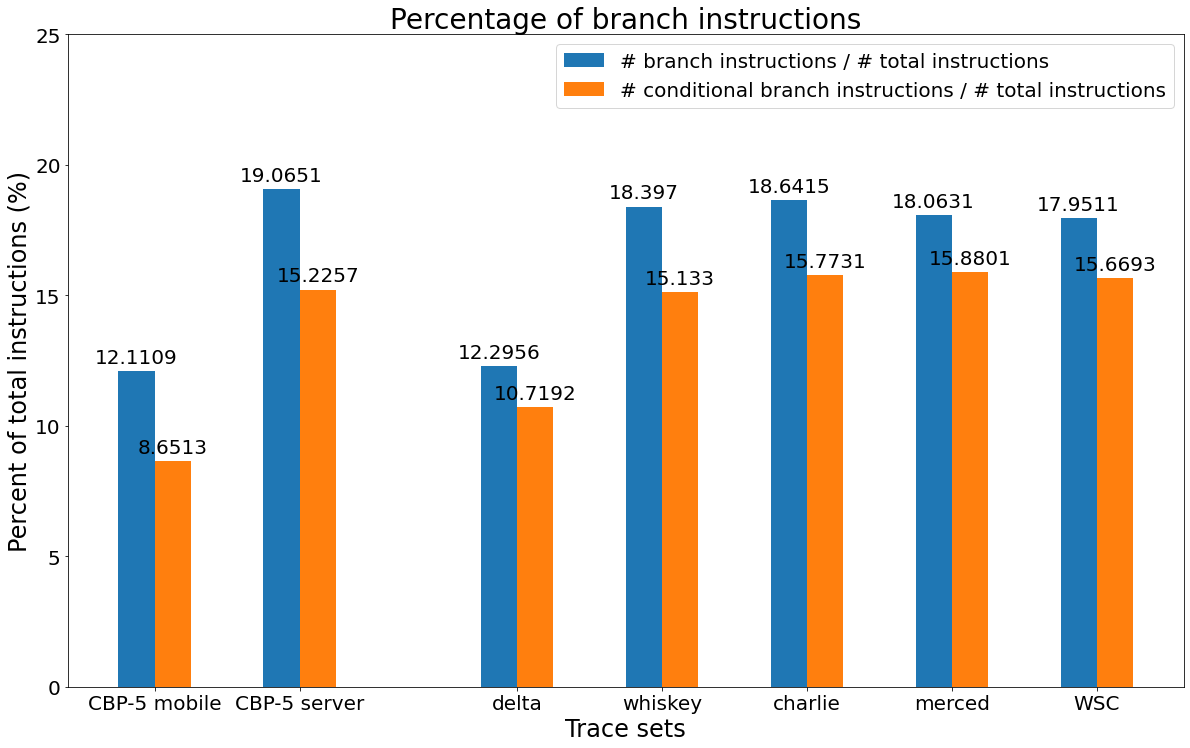
\includegraphics[width=0.8\textwidth]{Chapter3/Figs/br percent.png}
\caption{\centering Branch instruction and conditional branch instruction percent}
\label{fig:branchinstfrac}
\end{figure} % branch inst fraction plot


\subsubsection{Fraction of branch instructions}

As this project focused on conditional branch only, the proportions of branch instruction and conditional branch instructions are studied first Figure~\ref{fig:branchinstfrac}. The proportions of both branch instructions and conditional branch instructions in WSC sets are almost equal to those in CBP-5 \textit{server} and higher than in CBP-5 \textit{mobile}, suggesting a higher similarity between WSC and CBP-5 \textit{server} than CBP-5 \textit{mobile}. Also note that \textit{delta} have fewer branch instructions and conditional branch instructions than other WSC sets, which is one of the major causes why \textit{delta} has the smallest MPKI among the WSC sets. \par\hspace*{\fill}\par



Besides, 0.00127\% instructions are \textit{interrupt} and 0.00142\% instructions are \textit{context switch} in WSC sets.
This verifies the previous assumption in Section~\ref{interrupt} that \textit{interrupt} and \textit{context switch} take small proportion of the sets and that ignoring them has a negligible effect on the simulation results.
\label{frantion of interrupt}

\subsubsection{Trace lengths}

\begin{figure}[h!] 
\centering    
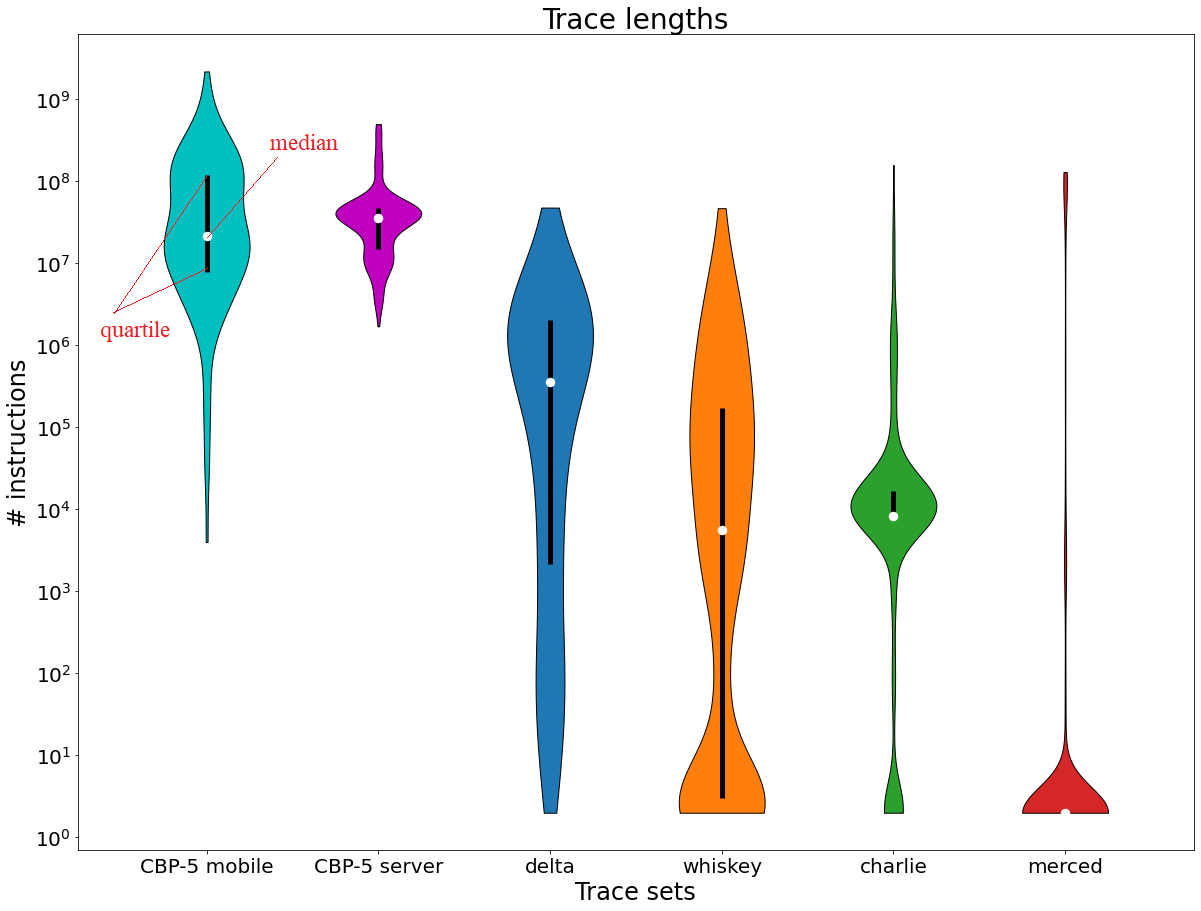
\includegraphics[width=0.8\textwidth]{Chapter3/Figs/tracelength.png}
\caption{\centering Trace lengths of six trace sets}
\label{fig:tracelength}
\end{figure} % trace length plot

In this report, since both CBP-5 and WSC traces show similar proportions of branch instruction, trace length is defined as the number of all types of instructions in a trace. Figure~\ref{fig:tracelength} shows the trace length distribution of each trace set, where the vertical coordinates indicate the trace length and each violin plot represents a set, with wider indicating more traces locate at the corresponding length.\par\hspace*{\fill}\par

While 90\% CBP-5 traces longer than $10^6$ instructions, WSC traces are significantly shorter and less concentrated with many traces even shorter than 100 instructions (particularly \textit{whiskey} and \textit{merced}). Since Google Workload Traces\cite{noauthor_google_nodate} are raw data directly captured from the machine and each trace represents a software thread, we presume very short traces represent idle threads while the program is running. As the predictors require a learning process, too short traces do not reflect the prediction accuracy of the predictor, and an example is thousands of traces containing only 16 instructions reporting an MPKI of 62.5, well above the MPKI reported by other long traces. 

\subsubsection{Uniting traces}

Since short traces contribute unreasonably high MPKIs but have very limited impact on actual system performance, the default methods of CBP-5 that counts the MPKI of all traces and calculate the arithmetic mean for each set is no longer reasonable for Google Workload Traces. Three new solutions were proposed to overcome this problem: 

\begin{enumerate}[itemsep= 0pt,topsep = 0pt, partopsep=4 pt, leftmargin= 32 pt]
\item Filter traces shorter than a certain length 
\item \textbf{Unite all the traces in a set after the simulation. }
\item Do not reset the predictor between traces in the same set.
\end{enumerate}

\hspace*{\fill}\par
Confirmed with Google, this solution 2 is supported by the fact that all traces within the same trace set are for the same run of the application, therefore share the address space. In a set if two branches occurring in different traces share same virtual address they are recognised as same unique branch, thus the total executed number and misprediction number within a set can be obtained for each unique branch, and this is called "uniting traces" in this report. In solution 2, each trace is still simulated independently and the MPKI is calculated after uniting the simulation results of all the traces in a set. Solution 1 requires a reasonable criteria to filter traces which we do not currently have and solution 3 is time consuming, requiring additional code and another simulation. Given the limited project duration, solution 2 is applied and WSC traces are united within each sets.\par\hspace*{\fill}\par

One of the idea raised from uniting WSC traces is can CBP-5 traces also be united? This idea is objected by Table~\ref{table:unite CBP}, whose first row represents the number of UBs in each set and second row is obtained directly adding up the number of UBs in each individual trace). The third row shows the ratio of the first row to the second row, it is called commonality ratio and it reflects the proportion of branches that are shared by different traces within a set; the lower the commonality ratio, the more likely it is that the set of traces was captured under a single launch. Both CBP-5 sets have a much higher commonality ratio than WSC traces, implying that they are less likely captured under same software launch.\par\hspace*{\fill}\par

Comparing the united mean of WSC sets with the arithmetic mean of CBP-5 may be questioned to be unscientific. However, the CBP-5 traces are parallel and independent with each other so it is logically to calculate their arithmetic mean; whereas the traces in a WSC set are captured under a single launch, contain complex interconnections and are not equivalent (some threads carry the main workload) so it is reasonable to introduce weight by uniting traces.

\begin{table}[h!] 
\centering
\begin{tabular}{l r r r r r r}
\toprule{\LARGE}
\multirow{2}{*}{} & \multicolumn{2}{c}{CBP-5} & \multicolumn{4}{c}{Google Workload Traces} \\ 
\cmidrule{2-3} \cmidrule{4-7}
  & \textit{mobile} & \textit{server}  & \textit{delta} & \textit{whiskey} & \textit{charlie} & \textit{merced}  \\ 
\midrule
\# unique branches (UBs)     & \sout{152K}   & \sout{456K}  & 63K  & 904K  & 499K & 290K  \\

\# adding up UBs  & 444K   & 2,234K  & 1,088K  & 10,481K  & 20,035K  & 56,328K \\

commonality ratio         & 34.3\% & 20.4\%  & 5.81\% & 8.63\%  & 2.49\%  & 0.515\% \\

\# average UBs (top 6) & 35.5K & 82.7K & 23.0K & 166.5K & 282.1K & 133.1K \\

\bottomrule
\end{tabular}
\caption{\centering \small Commonality reatio \& Average UBs (top 6). The commonality ratio reflects the proportion of branches that are shared by different traces within a set; the lower the ratio, the more likely it is that the set of traces was captured under a single launch.}
\label{table:unite CBP}
\end{table} % Uniting trace verification

\subsubsection{Number of unique branches (UBs)}

The reason for the interest in the number of UBs is because of Aliasing. Aliasing is a well-known phenomenon that affects predictor accuracy by limiting the predictor's ability to accurately identify UBs. Due to the limited capacity of the predictor, a great amount of UBs in a trace can put high pressure on the predictor capacity, thus causing aliasing and reducing predictor accuracy.\par\hspace*{\fill}\par

Considering the large number of short traces in WSC sets, the average of the six traces with the most UBs are calculated and appended to Table~\ref{table:unite CBP}. According to the averaged UBs, \textit{server} has two times more than \textit{mobile}, in line with the simulation results where the MPKI of \textit{server} is more than twice that of the \textit{mobile}. Most WSC traces (i.e. except \textit{delta}) have 1.6-3.4 times more UBs than \textit{server}, implying a much higher MPKI than \textit{server} can be expected (though this is not the case, as discussed in Section~\ref{MPKI results}). \par\hspace*{\fill}\par

As to \textit{delta}, not like other WSC sets, it has less UBs than \textit{mobile}, implying that its MKPI can be even lower than mobile (verified by the simulation result). Besides, the great variation between WSC applications is again confirmed: delta looks more like \textit{mobile} than a WSC set.


\subsubsection{Fraction of unidirectional unique (UU) branches}

Unidirectional unique branches (UDUBs) are of particular interest because they have only one choice (T or N) and are easy to predict while occupying the same amount of resources as other more complex UBs under the present predictor schemes. Research on them may help optimize predictor designs for UU branches to saving valuable capacity. Since uniting is not valid for CBP-5 sets, six traces with the largest number of UBs are selected and averaged (Table~\ref{table:selected CBP-5}) for both CBP-5 \textit{mobile} and CBP-5 \textit{server}. The fraction of taken UU branches, not-taken UU branches, their summation and the ratio of taken UU branches to not-taken UU branches are obtained for selected CBP-5 traces and united WSC sets.

\begin{table}[h!] 
\vskip 0.2in
\centering
\begin{tabular}{c c c c c c}
\toprule{\LARGE}
\multirow{2}{*}{} & \multicolumn{2}{c}{\textit{mobile}} & \multicolumn{2}{c}{\textit{server}} &\\ 
\cmidrule(l{3pt}r{3pt}){2-3} \cmidrule(l{3pt}r{3pt}){4-5}
&trace name & \# UBs & trace name & \# UBs  \\ 
\midrule
&SHORT\_MOBILE-33 & 41984 & SHORT\_SERVER-5 & 89864\\
&LONG\_MOBILE-14 & 38832 & LONG\_SERVER-2.res & 89864\\
&SHORT\_MOBILE-32 & 36949 & SHORT\_SERVER-6.res & 88689\\
&SHORT\_MOBILE-35 & 33592 & LONG\_SERVER-3.res & 88689\\
&SHORT\_MOBILE-36 & 30839 & SHORT\_SERVER-8 & 69612\\
&LONG\_MOBILE-15 & 30839 & LONG\_SERVER-4.res & 69612\\
\bottomrule
\end{tabular}
\caption{\centering \small Selected CBP-5 traces with the largest number of unique branches (UBs)}
\label{table:selected CBP-5}
\end{table} % Table: selected CBP-5


It's clearly shown in Table~\ref{table:UU Branches} that the fraction of UU branches are similar and about 80\% for both CBP-5 and WSC, hinting at the potential for optimisation for UU branches. Whoever the ratio of taken UU branches to not-taken UU branches are significantly different in CBP-5 and WSC. Depending on different WSC sets not-taken UU branches can be 5~12 times more than taken UU branches, compared with 1.5 times for \textit{mobile} and 2.1 times for \textit{server}. More not-taken UU branches indicate that WSC is a stronger biased workload, which reduces the direction prediction difficulty. Another point worth mentioning is that the WSC still show significant differences about UU branches between sets: \textit{merced} has the smallest proportion of UU branches while \textit{whiskey} has the largest.\par\hspace*{\fill}\par


In contrast to UU branches, hart-to-predict (HTP) branches are also of interest and are discussed this in later sections.

\begin{table}[h!] 
\centering
\vskip 0.2in
\begin{tabular}{l r r r r r r}
\toprule{\LARGE}
\multirow{2}{*}{} & \multicolumn{2}{c}{CBP-5} & \multicolumn{4}{c}{Google Workload Traces} \\ 
 \cmidrule(l{3pt}r{3pt}){2-3} \cmidrule(l{3pt}r{3pt}){4-7}
  & \textit{mobile} & \textit{server}  & \textit{delta} & \textit{whiskey} & \textit{charlie} & \textit{merced}  \\ 
\midrule
Taken UU branches      & 30.42\%   & 25.90\%    & 6.25\%  & 12.31\%  & 9.38\%   & 6.43\% \\

Not-taken UU branches   & 46.40\%   & 54.39\%  & 73.51\%  & 70.16\%  & 68.44\%  & 62.10\% \\

All UU branches         & 76.82\%   & 82.83\%  & 79.75\%  & 82.46\%  & 77.82\%  & 68.53\% \\

Not-taken / Taken         & 1.536     & 2.101    & 11.77    & 5.700    & 7.298    & 9.653   \\
\bottomrule
\end{tabular}
\caption{\centering \small Fraction of unidirectional unique branches (UDUBs). CBP-5 data is obtained from six selected traces, while WSC data is obtained from united WSC sets.}
\label{table:UU Branches}
\end{table} % Table: UU Branch


\section{Impact of trace sets on MPKI}

The simulation results are discussed in this section, mainly around the differences between trace sets. Despite the high pressure put on the predictors' capabilities by the large number of UBs, the WSC sets reports MPKIs that are similar to or even slightly lower than the MPKI of \textit{server}. This result means that due to specific tasks and similar context\cite{barroso_datacenter_2013} WSC is a more predictable workload. Note that WSC sets continue to show a huge variation in simulation results, emphasising the importance of application-specific analysis.\par\hspace*{\fill}\par

The MPKI are shown in Figure~\ref{fig:MPKI}. Contrary to previous expectation, MPKI of united WSC is 15.7\% lower than server, suggesting that there are other factors increase WSC prediction accuracy (e.g. very few applications or large fraction of not-taken UDUBs). Since WSC sets are highly differentiated, all sets are shown in Figure~\ref{fig:Normalized MPKI}. Normalizing sets to server is to compare the adaptability of different predictors to WSC in later section. MPKI proves that \textit{whiskey, charlie} and \textit{merced} put higher pressure on predictor capacity than \textit{delta}, due to much more UBs.\par\hspace*{\fill}\par


The paradox of WSC sets (except \textit{delta}) having more UBs but lower MPKI than \textit{server} suggests that WSC has some features makes branches highly predictable, which is in line with previous summaries of WSC features from a higher level. Despite WSC sets have more UBs, they also have more not-taken UUBs (thus strongly biased), more specific application and larger-scale parallel instruction context. \par\hspace*{\fill}\par

\begin{figure}[h!] 
     \centering
     \begin{subfigure}{1\textwidth}
         \centering
         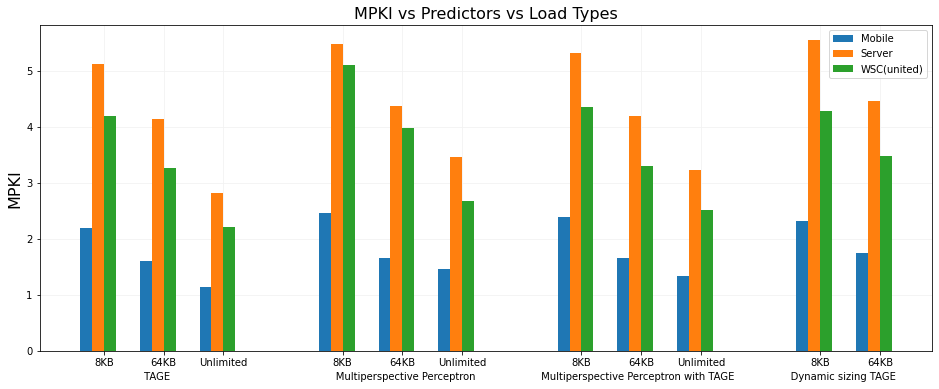
\includegraphics[width=1.0\textwidth]{Chapter3/Figs/MPKI vs Predictors vs Load Types.png}
         \caption{MPKI vs Predictors vs Load Types}
         \label{fig:MPKI}
     \end{subfigure}
     \newline
     \begin{subfigure}{1\textwidth}
         \centering
         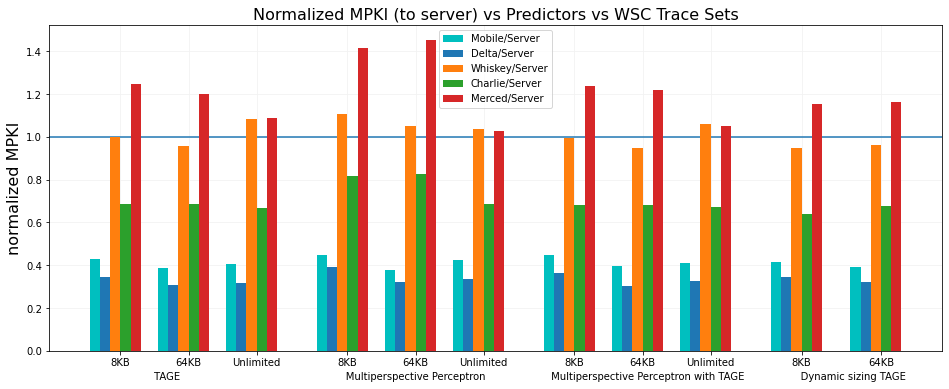
\includegraphics[width=1\textwidth]{Chapter3/Figs/Normalized MPKI (to server) vs Predictors vs WSC Trace Sets.png}
         \caption{Normalized MPKI (to server) vs Predictors vs WSC Trace Sets}
         \label{fig:Normalized MPKI}
     \end{subfigure}
        \caption{MPKI histograms \& Normalized MPKI of 6 trace sets and 11 predictors }
        \label{fig:MPKI histograms}
\end{figure} % MPKI plot
\label{MPKI results}



\newpage
% Section 3.3 Simulation results between predictors % Section 3.2 Simulation results between sets
\section{Impact of predictors on MPKI}

Figure~\ref{fig:MPKI histograms} shows MPKI of all predictor. On WSC sets, TAGE scheme (TAGE-SC-L \& MTAGE-SC) is still SOTA, followed by the Multiperspective Perceptron Predictor with TAGE (MPP-TAGE) and Dynamically sized TAGE (DS-TAGE). The multiperspective perceptron predictor (MPP) reports highest MPKI on all capacities. While DS-TAGE reports higher MPKI than MPP on \textit{server}, DS-TAGE reversed the results on WSC. This draws attention to the variation of each predictor in server and WSC, thus that the normalized MPKI is plotted. 8KB \& 64KB MPP has the largest normalised MPKI and worst adaptation on WSC, resulting in the highest MPKI. However, Unlimited MPP has the smallest normalised MPKI, suggesting that large MMP has the potential to do well on WSC traces. Besides, For all predictors schemes and most WSC sets, unlimited versions report smaller normalised MPKI, because the impact of UBs increasing is less significant for unlimited capacity.


\section{Hard-to-predict branches (HTPB)}

Hard-to-predict branches are those unique branches that hard to predict and contribute to the most of misprediction. By sorting unique branches using the number of mispredictions and ploting the accumulated misprediction percent, Figure~\ref{fig:HTP branches vs WSC sets} are plotted. A horizontal line is placed at 90\% mispredictions to help count how many unique branches contribute 90\% mispredictions to the whole set. This number is defined as the number of HTPB in this project. Four predictors are selected such that three of them are TAGE with different size, and one of them is 64KB MPP-TAGE to campare with 64KB TAGE-SC-L.\par\hspace*{\fill}\par

Firstly, significant variation is still observed for four WSC sets. The number of HTPB generally increase with number of UUBs, but still affected by specific feature of individual set. The more HTPB there are in a set, the larger capacity is required to address those HTPB.\par\hspace*{\fill}\par

Secondly, the numbers of HTPB do not change significantly with predictors, but are suddenly reduced when unlimited capacity is applied. This indicates how many unique branches are hard to be predicted by the current scheme, ignoring the limitation from the predictor size.


\begin{figure}[h!] 
     \centering
     \begin{subfigure}{0.45\textwidth}
         \centering
         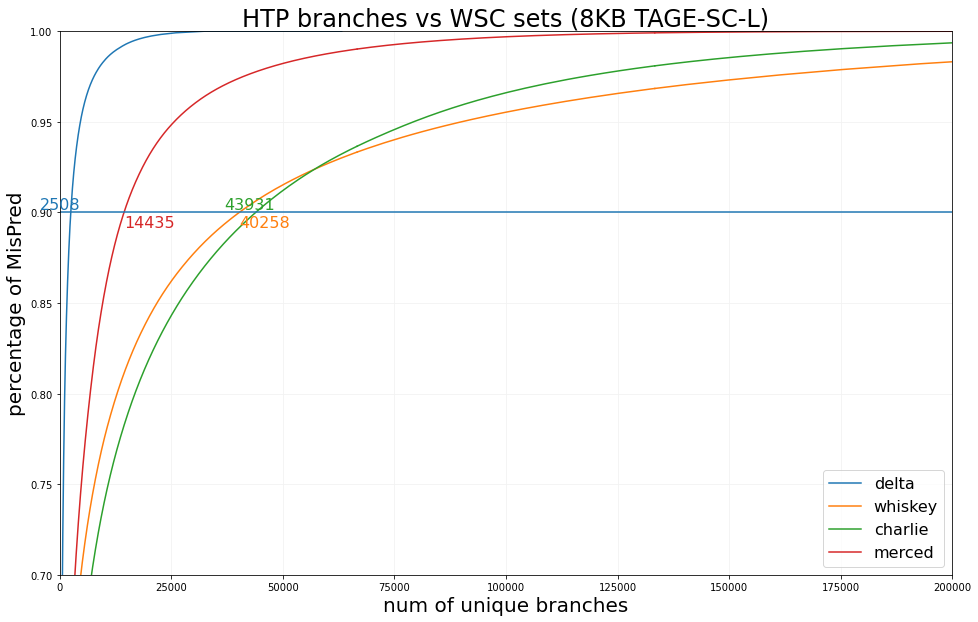
\includegraphics[width=1\textwidth]{Chapter3/Figs/HTP branches vs WSC sets (8KB TAGE-SC-L).png}
         \caption{8KB TAGE-SC-L}
         %\label{fig:MPKI}
     \end{subfigure}
     \begin{subfigure}{0.45\textwidth}
         \centering
         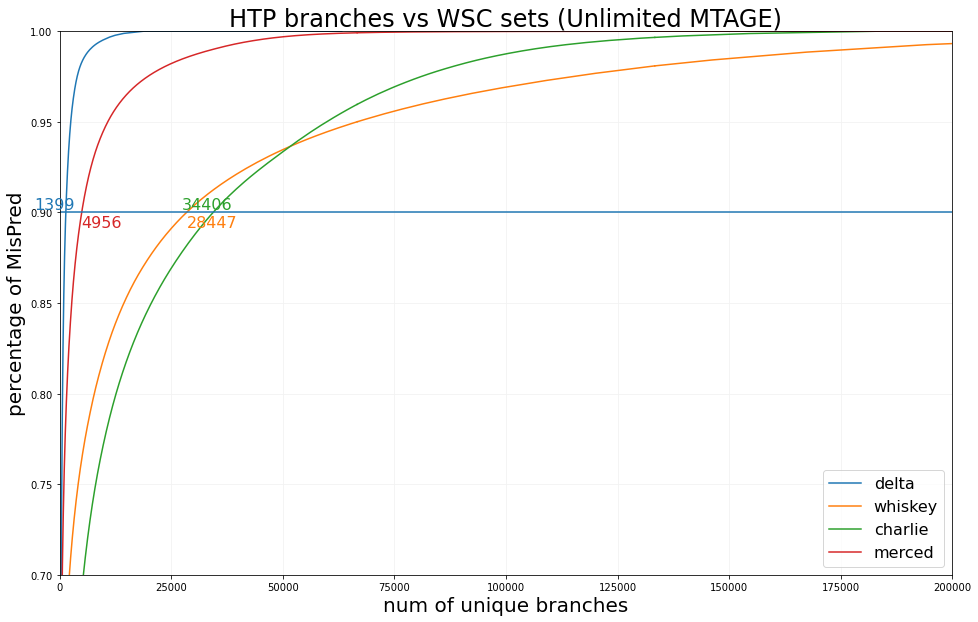
\includegraphics[width=1\textwidth]{Chapter3/Figs/HTP branches vs WSC sets (Unlimited MTAGE) (2).png}
         \caption{Unlimited MTAGE-SC}
         %\label{fig:MPKI}
     \end{subfigure}
     \hfill
     \begin{subfigure}{0.45\textwidth}
         \centering
         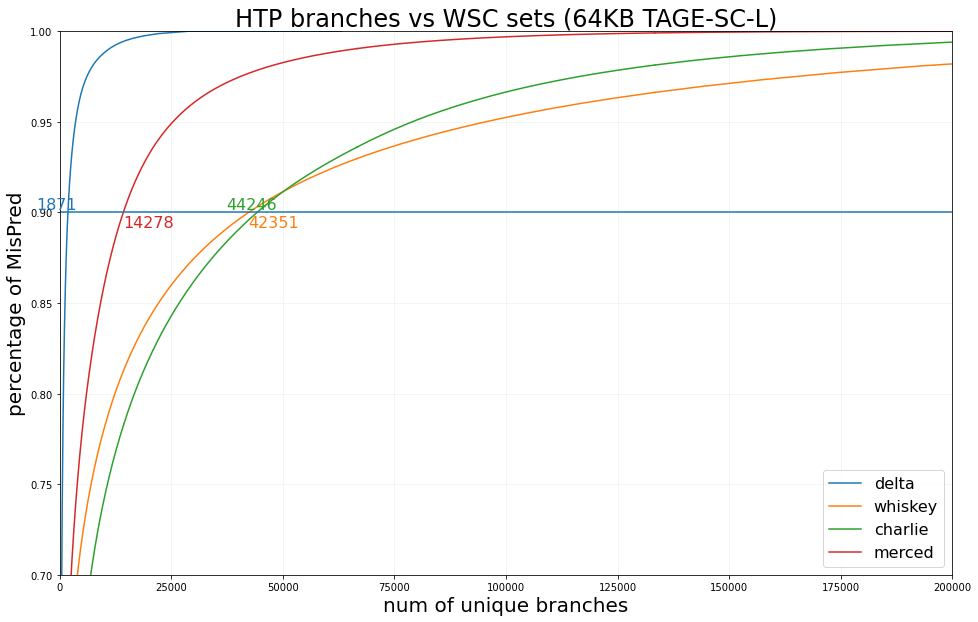
\includegraphics[width=1\textwidth]{Chapter3/Figs/HTP branches vs WSC sets (64KB TAGE-SC-L).png}
         \caption{64KB TAGE-SC-L}
         %\label{fig:Normalized MPKI}
     \end{subfigure}
     \begin{subfigure}{0.45\textwidth}
         \centering
         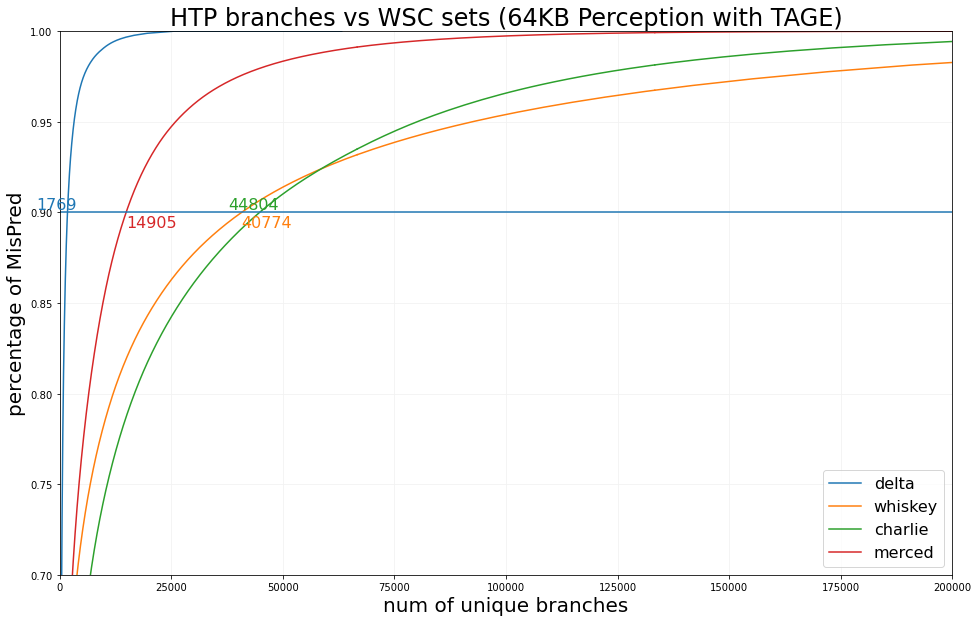
\includegraphics[width=1\textwidth]{Chapter3/Figs/HTP branches vs WSC sets (64KB Perception with TAGE).png}
         \caption{64KB Perception with TAGE (MPP-TAGE)}
         %\label{fig:Normalized MPKI}
     \end{subfigure}
     
\caption{HTP branches vs WSC sets}
\label{fig:HTP branches vs WSC sets}
\end{figure} % MPKI plot
\label{MPKI results}

\newpage
\section{Discussion of the results}
\label{result discussion}

\begin{figure}[h!] 
\centering    
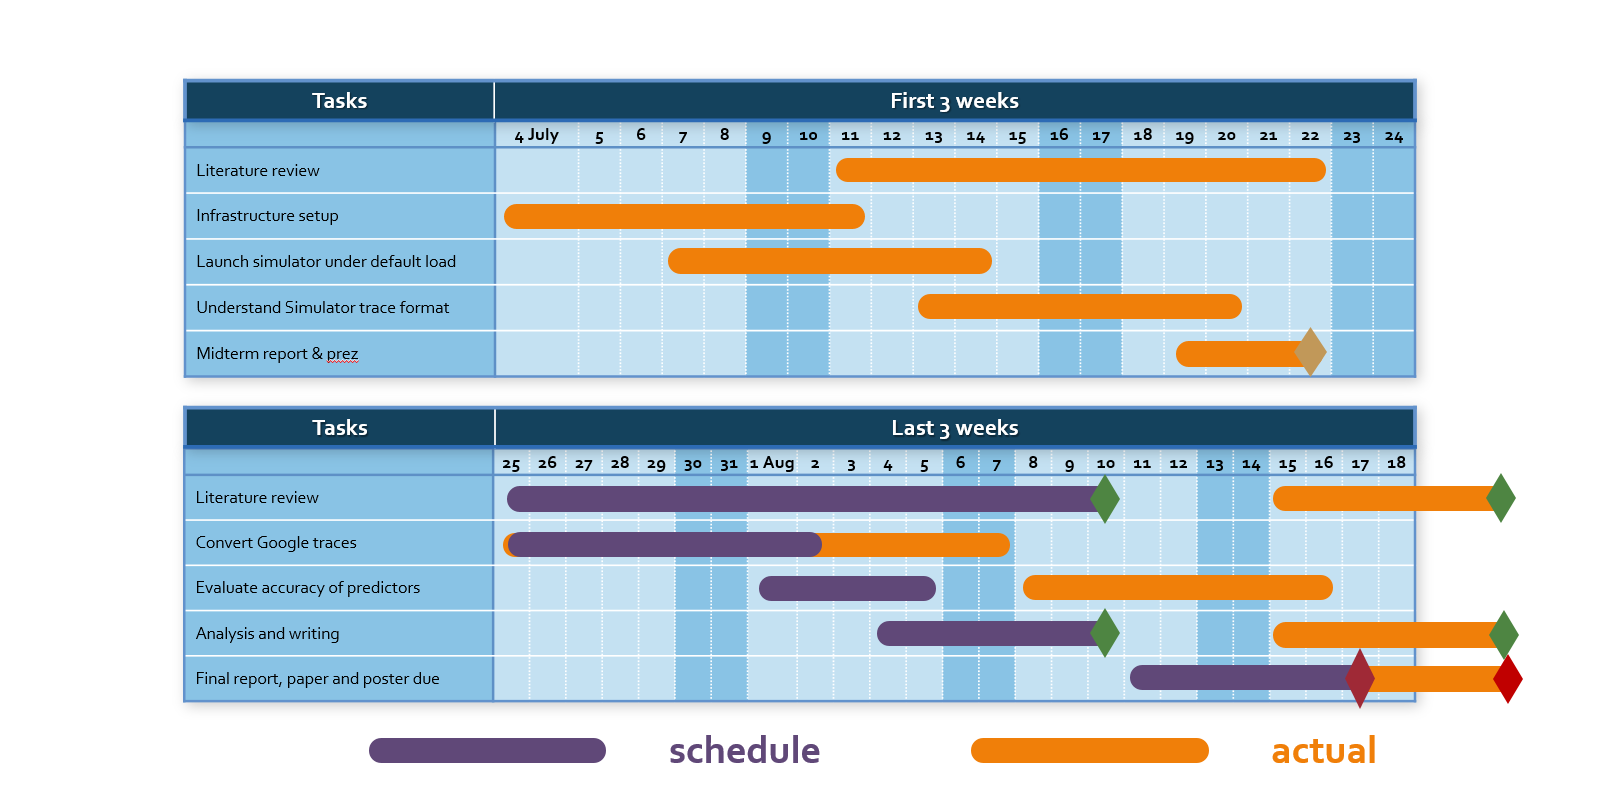
\includegraphics[width=1\textwidth]{Chapter3/Figs/final gantt chart.png}
\caption{\centering Project progress Gantt Chart}
\label{fig:gantt chart}
\end{figure}

Shown in the final gantt chart (Figure~\ref{fig:gantt chart}), the results of the project are generally acceptable and all planned objectives have been completed. Unexpected problems were encountered in two main areas, resulting in delays of the project:

\begin{enumerate}[itemsep= 0pt,topsep = 0pt, partopsep=4 pt, leftmargin= 32 pt]
\item Mismatch between the information provided by Google Workload Traces and expected by CBP-5 simulator.
\item Raw, unprocessed trace sets from Google Workload Traces.
\end{enumerate}

\hspace*{\fill}\par
Problems caused by the former include type, behaviour and size problem as discussed in Section~\ref{BT9 Converson}. Though having been mostly addressed but the start of the simulation was postponed by a week from schedule because of them. The second aspect was only realised towards the end of the project, when the limited time available meant that we could only process the simulation data as much as possible (uniting traces) and could not re-simulate it after processing the raw trace.\par\hspace*{\fill}\par

Overall, the project has some points for improvement in the future. Firstly, pre-processing of the WSC raw data is desired. Uniting the WSC sets into one trace before simulation or modifying the simulator to avoid resetting of predictors between traces within the same set are both acceptable. Secondly, the calculation of the commonality ratio is not rigorous because it has high dependency on the number of traces in the analysed set. A better way to check the validity of uniting CBP-5 traces is to calculate pair-based commonality ratio and then average on the whole set. Or even simpler - contact the CBP-5 organizer to get confirmation. Finally, limited to the understanding on branching prediction, this project does not adequately compare and analyse the prediction accuracy of the various predictors.
